% Propósito: seguir la transformación desde una presión acústica local hasta
% un nivel informado por un sonómetro y distinguir señal física, procesamiento
% y resultado.
% Origen: cadena funcional conceptual descrita en la sección Sonómetro de la
% Unidad 5. No representa la arquitectura interna de un modelo comercial ni
% especifica requisitos normativos.
% Descripción accesible: seis bloques conectados muestran micrófono,
% preamplificación y conversión, ponderación frecuencial, detector o integrador,
% ponderación temporal, y visualización y almacenamiento. La entrada es presión
% acústica en pascales; la salida es un nivel acompañado por su ponderación e
% intervalo temporal.
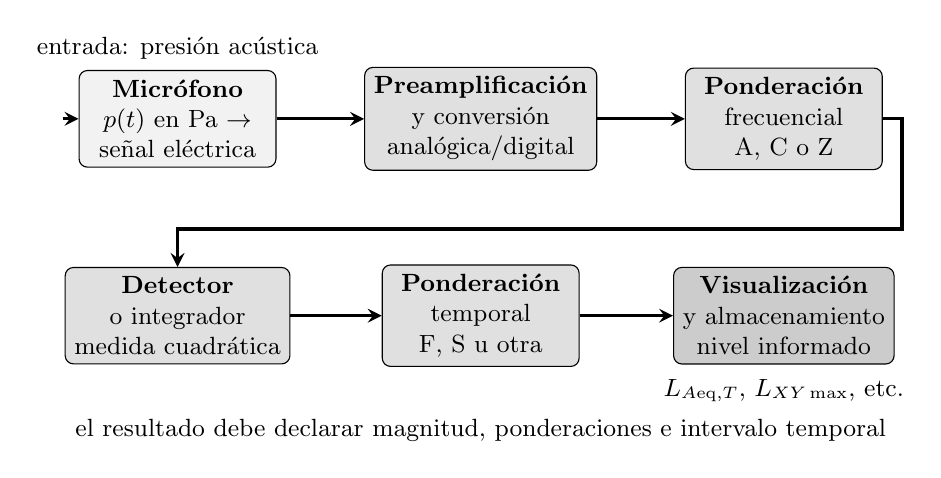
\begin{tikzpicture}[font=\small,>=stealth,x=1cm,y=1cm]
    \tikzset{
        block/.style={
            draw,
            rounded corners=3pt,
            minimum width=2.50cm,
            minimum height=1.10cm,
            align=center
        },
        signal/.style={block,fill=black!5},
        process/.style={block,fill=black!12},
        result/.style={block,fill=black!20}
    }

    \node[signal] (mic) at (1.45,3.15)
        {\textbf{Micrófono}\\
         \(p(t)\) en Pa \(\rightarrow\)\\señal eléctrica};
    \node[process] (pre) at (5.30,3.15)
        {\textbf{Preamplificación}\\
         y conversión\\analógica/digital};
    \node[process] (freq) at (9.15,3.15)
        {\textbf{Ponderación}\\
         frecuencial\\A, C o Z};

    \node[process] (det) at (1.45,0.65)
        {\textbf{Detector}\\
         o integrador\\medida cuadrática};
    \node[process] (time) at (5.30,0.65)
        {\textbf{Ponderación}\\
         temporal\\F, S u otra};
    \node[result] (display) at (9.15,0.65)
        {\textbf{Visualización}\\
         y almacenamiento\\nivel informado};

    \node at (1.45,4.05) {entrada: presión acústica};
    \draw[->,very thick] (0.00,3.15) -- (mic.west);
    \draw[->,very thick] (mic.east) -- (pre.west);
    \draw[->,very thick] (pre.east) -- (freq.west);
    \draw[->,very thick] (freq.east) -- (10.65,3.15)
        -- (10.65,1.75) -- (1.45,1.75) -- (det.north);
    \draw[->,very thick] (det.east) -- (time.west);
    \draw[->,very thick] (time.east) -- (display.west);
    \node[align=center] at (9.15,-0.30)
        {\(L_{A\mathrm{eq},T}\), \(L_{XY\max}\), etc.};

    \node[align=center] at (5.30,-0.80)
        {el resultado debe declarar magnitud, ponderaciones e intervalo temporal};
\end{tikzpicture}
